\documentclass[t]{beamer}

\usepackage[utf8]{inputenc}
\usepackage[T1]{fontenc}
%\usepackage{mathptmx}
\usepackage{helvet}
\usepackage[english]{babel}


%needed Package
\usepackage{wrapfig}
\usepackage{graphicx}
\usepackage{subfigure}
\usepackage{amssymb}
\usepackage{amsmath}		
\usepackage{booktabs}
\usepackage{smartdiagram}
\usepackage{threeparttable}
\usepackage{tikz}
\usetikzlibrary{positioning, shapes, arrows, calc, chains, scopes}
%\usepackage{caption}
\usepackage[justification=centering]{caption}
\usepackage{animate}

%bib
\usepackage{cite}
% Removes icon in bibliography
\setbeamertemplate{bibliography item}[text]

%theme
\usetheme{LUH}


%Title
\title{Theme or Title of the Project, Thesis}
\date[\today]{Hannover Centre for Optical Technologies, \today}
\author[Mustermann]{Muster Mustermann}
\institute[HOT]{Hannover Centre for Optical Technologies}
\unilogo{
\includegraphics[height=\LUHLogoHeight]{logo_luh.png}}
\logo{
\includegraphics[height=\LUHLogoHeight]{logo_hot.jpg}}
\titleimage{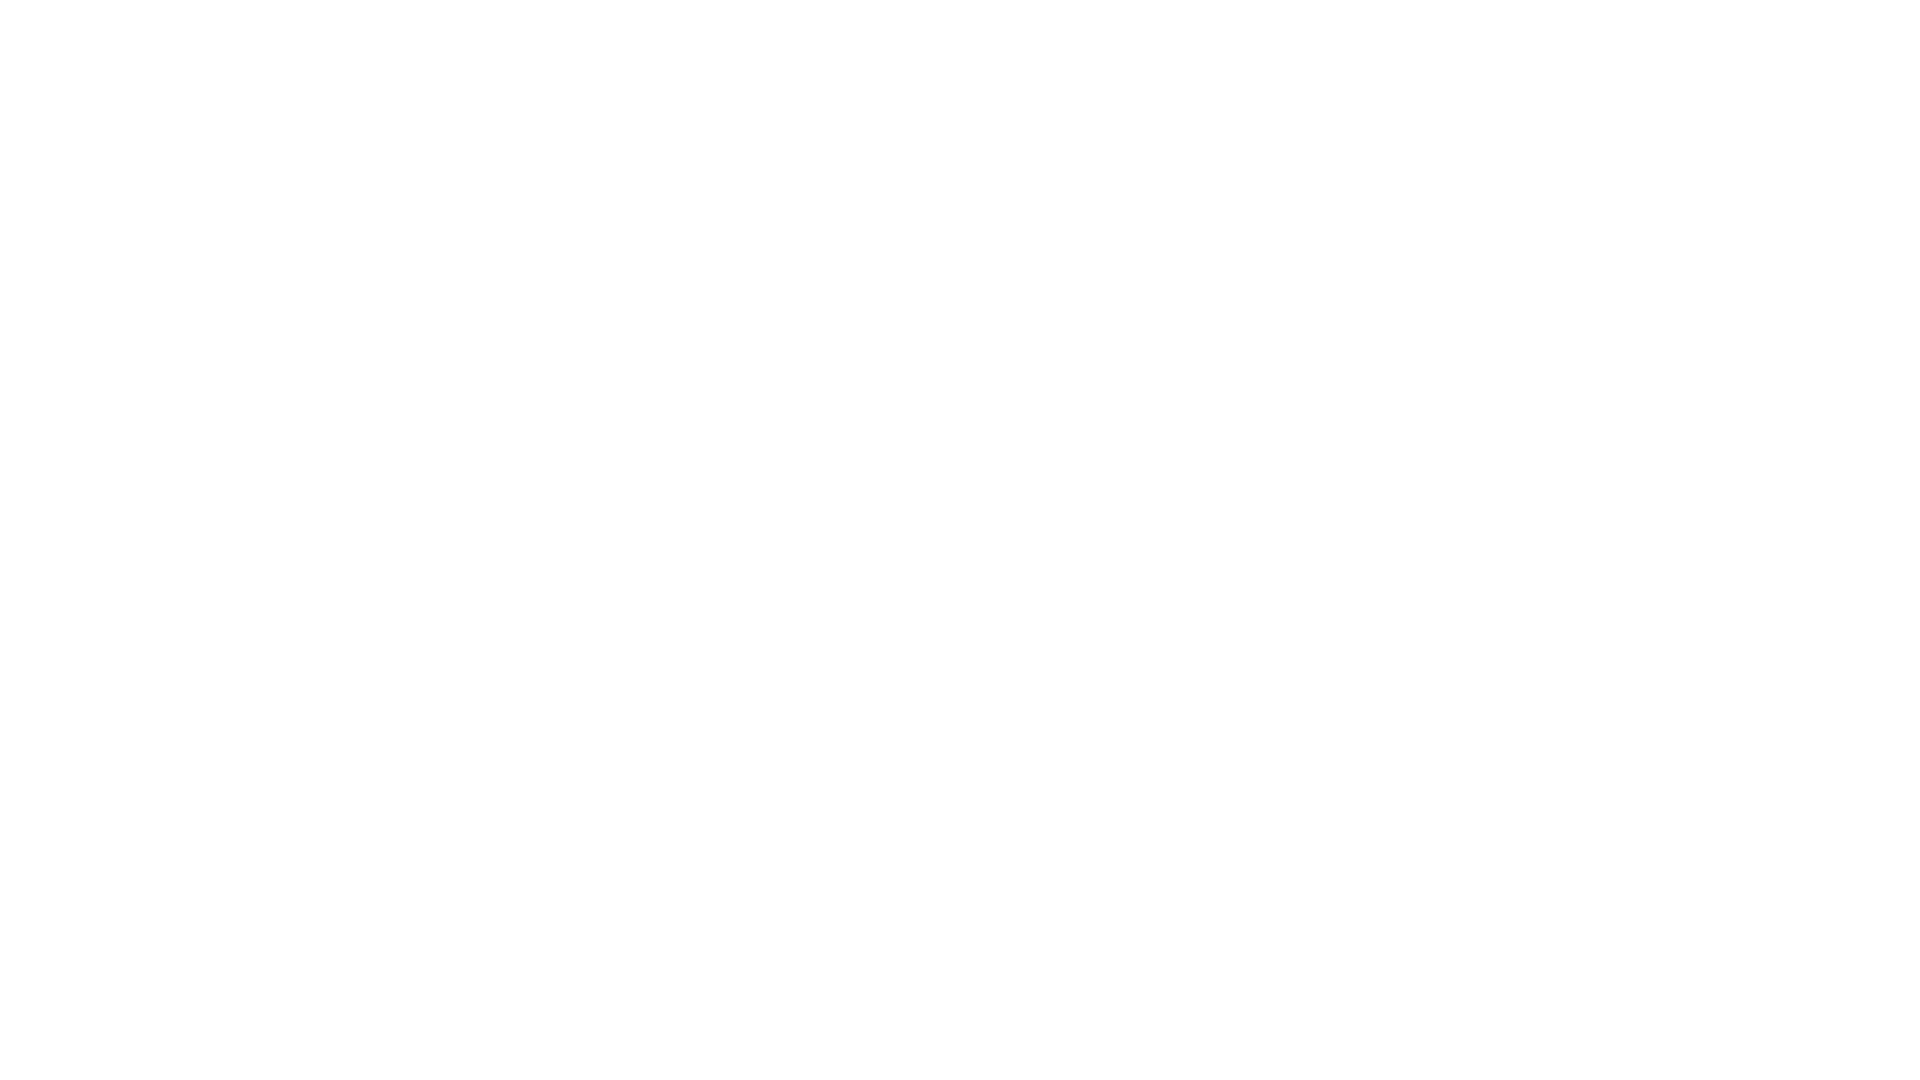
\includegraphics[width=.7\paperwidth]{logo_empty.png}}





\begin{document}

% Titleimage
\begin{frame}
\label{P1 Titlepage}
\titlepage
\end{frame}


% Content
\begin{frame}{Contents}
\label{P2 Content}

\begin{itemize}
  \item Introduction
    \begin{itemize}
        \item Introduction 1
	    \item Introduction 2
    \end{itemize}
    \item Theories
    \begin{itemize}
        \item Theories 1
	    \item Theories 2
	    \item Theories 3
    \end{itemize}
    \item Conclusion
    \item Outlook
\end{itemize}

\end{frame}


% New Frame
\begin{frame}{Introduction}
\framesubtitle{Introduction 1 - Section 1}
\label{P3 Introduction}

Section 1
\begin{itemize}
\item 111111111111;
\item 222222222222;
\item 333333333333;
\item 444444444444.
\end{itemize} 

\begin{minipage}[t]{.45\textwidth}
\centering
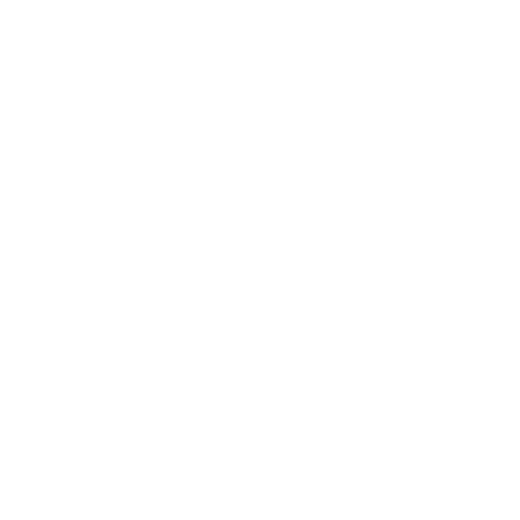
\includegraphics[width =25mm]{image/0}
\end{minipage}
\begin{minipage}[t]{.45\textwidth}
\centering
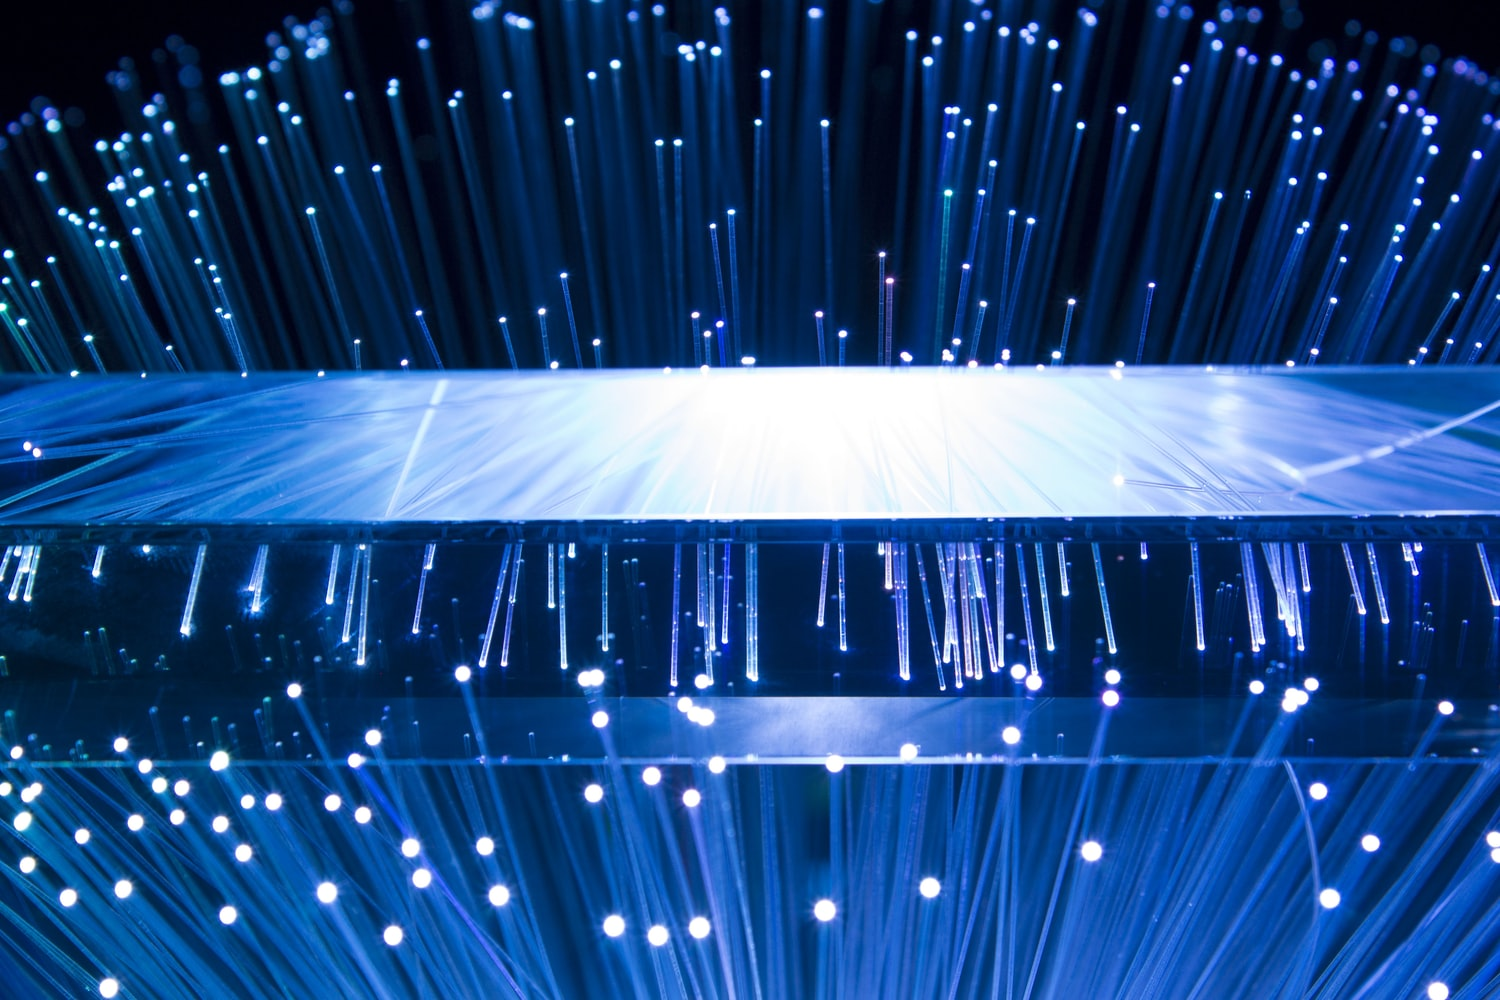
\includegraphics[width = 45mm]{image/a}
\captionof*{figure}{Wrapfig 1 \cite{knuth}}
\end{minipage}

\end{frame}


% New Frame
\begin{frame}{Introduction}
\framesubtitle{Introduction 2 - Section 1}
\label{P4 Introduction}

\begin{block}{Section 1.1}
    Section 1.1 Section 1.1 Section 1.1\cite{einstein}
\end{block}
\begin{block}{Section 1.2}
    Section 1.2 Section 1.2 Section 1.2
\end{block}

\end{frame}


% New Frame
\begin{frame}{Theories}
\framesubtitle{Theories 1}
\label{P5 Theories}

\begin{center}
    \begin{figure}[htbp]
        \centering
        \begin{minipage}[t]{0.3\textwidth}
            \centering
            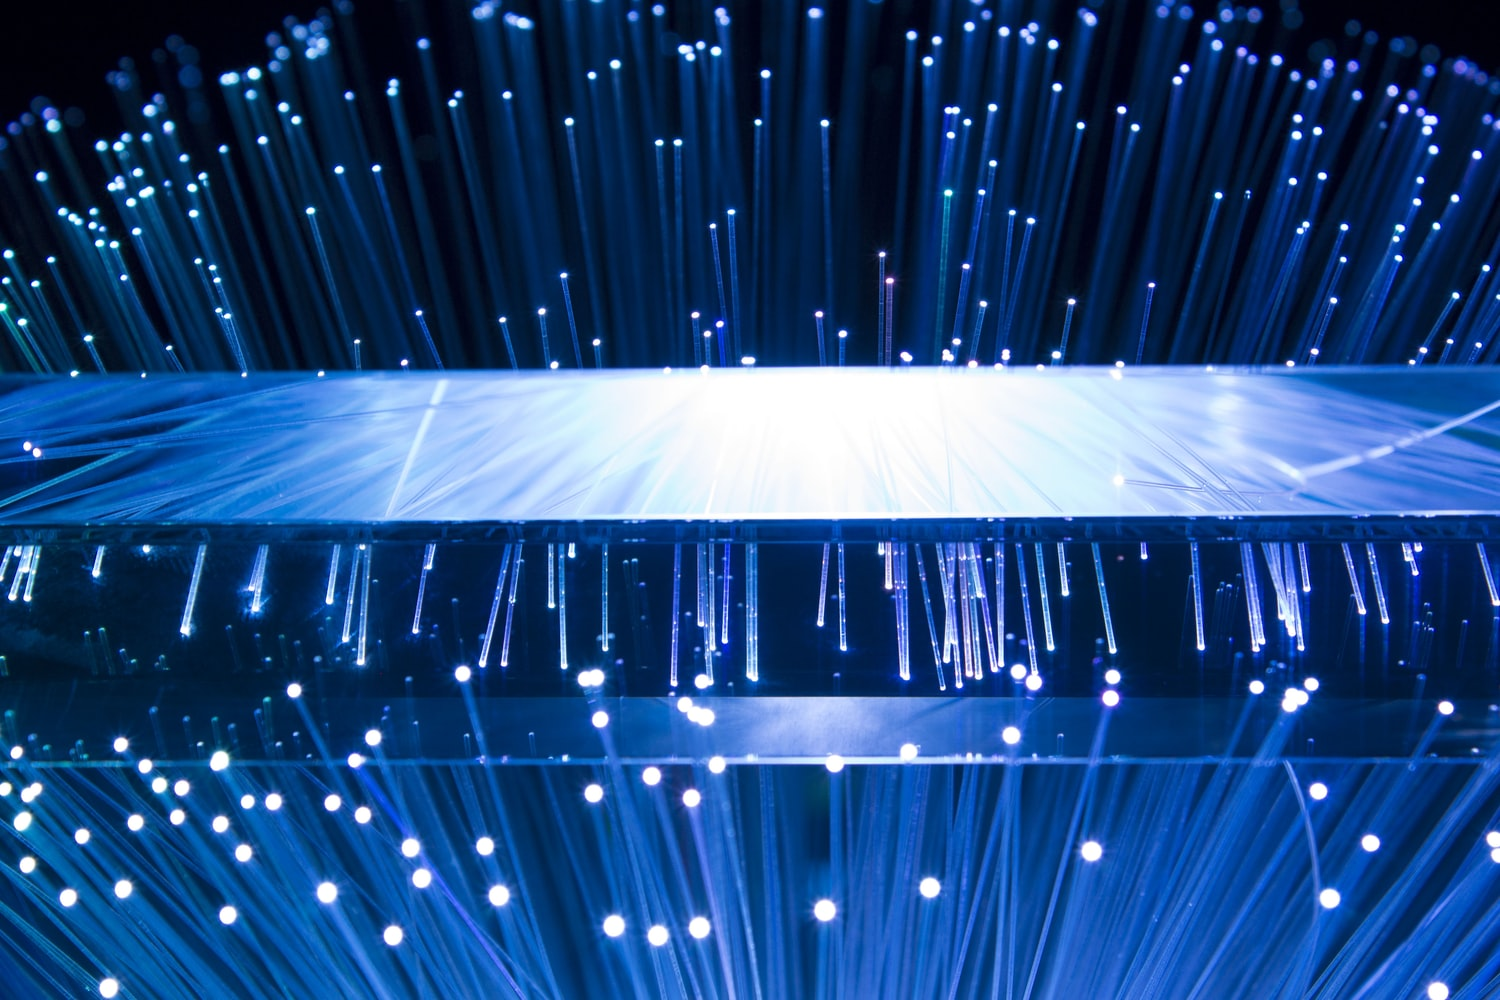
\includegraphics[width=\textwidth]{image/a}
                    \caption*{Figure a}
        \end{minipage}
    \hfill
        \begin{minipage}[t]{0.3\textwidth}
            \centering
            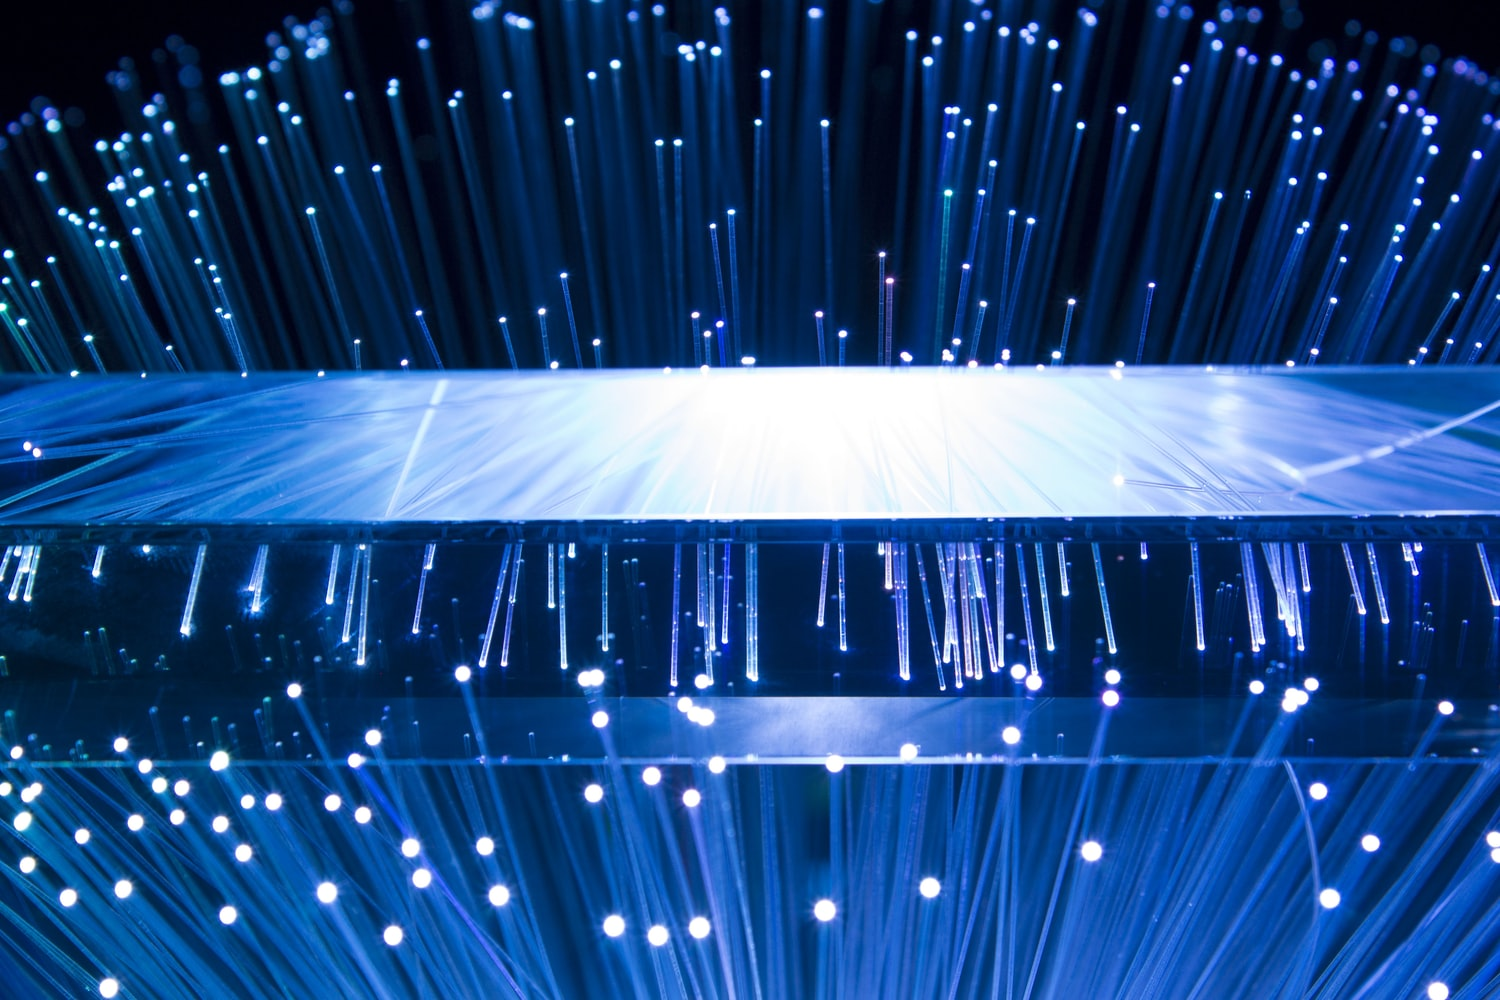
\includegraphics[width=\textwidth]{image/a}
                    \caption*{Figure a}
        \end{minipage}
    \hfill
        \begin{minipage}[t]{0.3\textwidth}
            \centering
            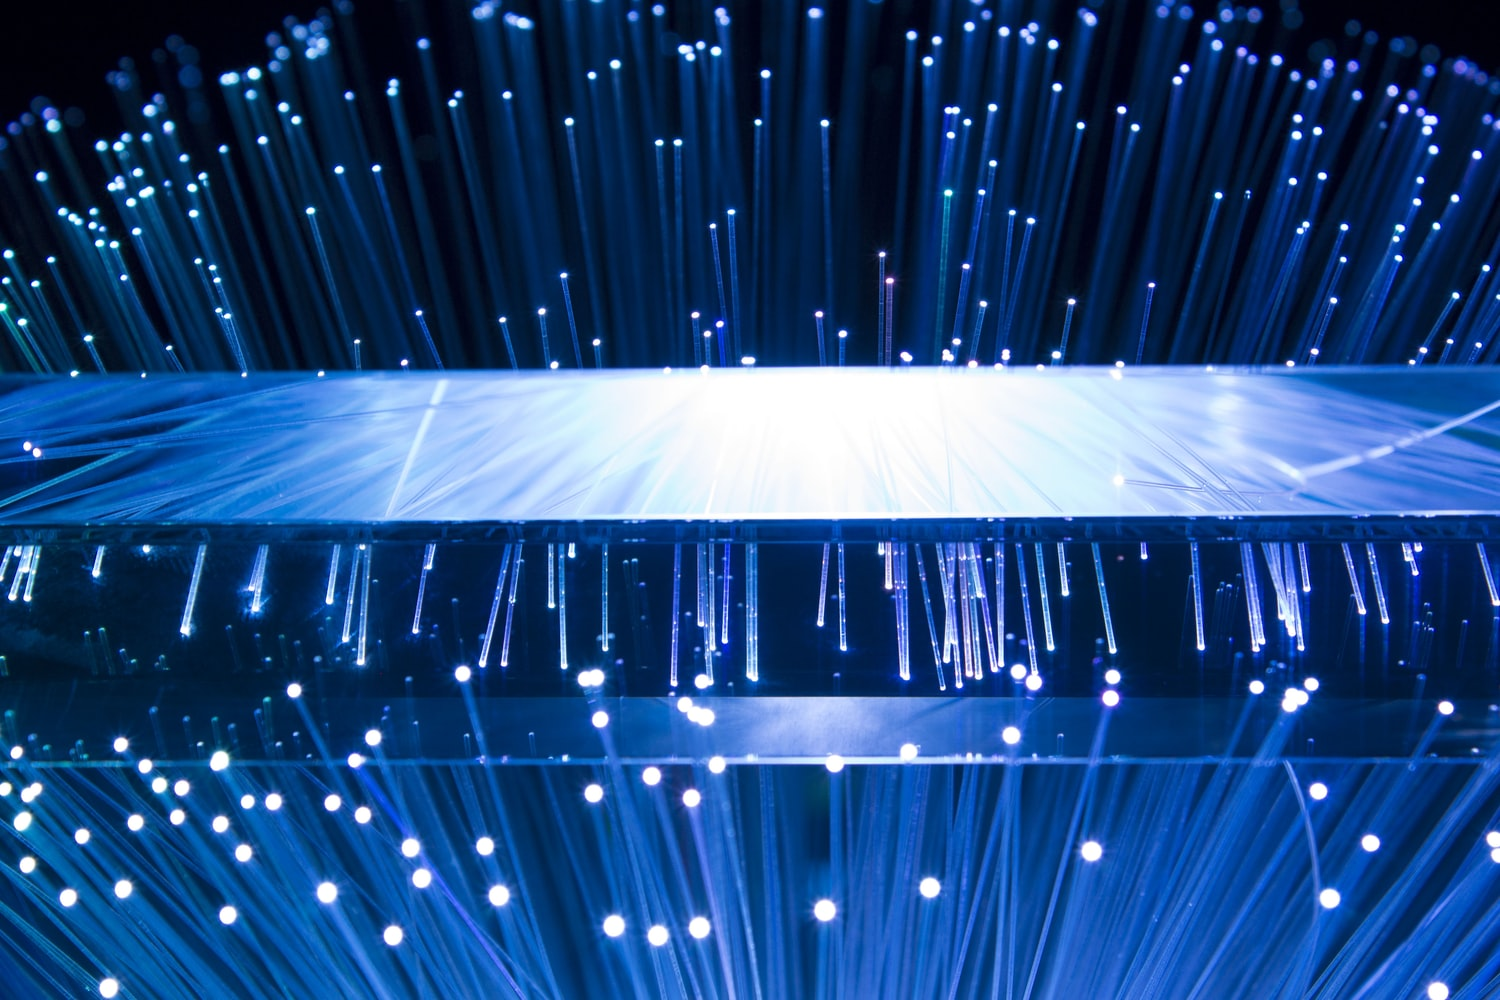
\includegraphics[width=\textwidth]{image/a}
                    \caption*{Figure a}
        \end{minipage}  
    \\
        \begin{minipage}[t]{0.3\textwidth}
            \centering
            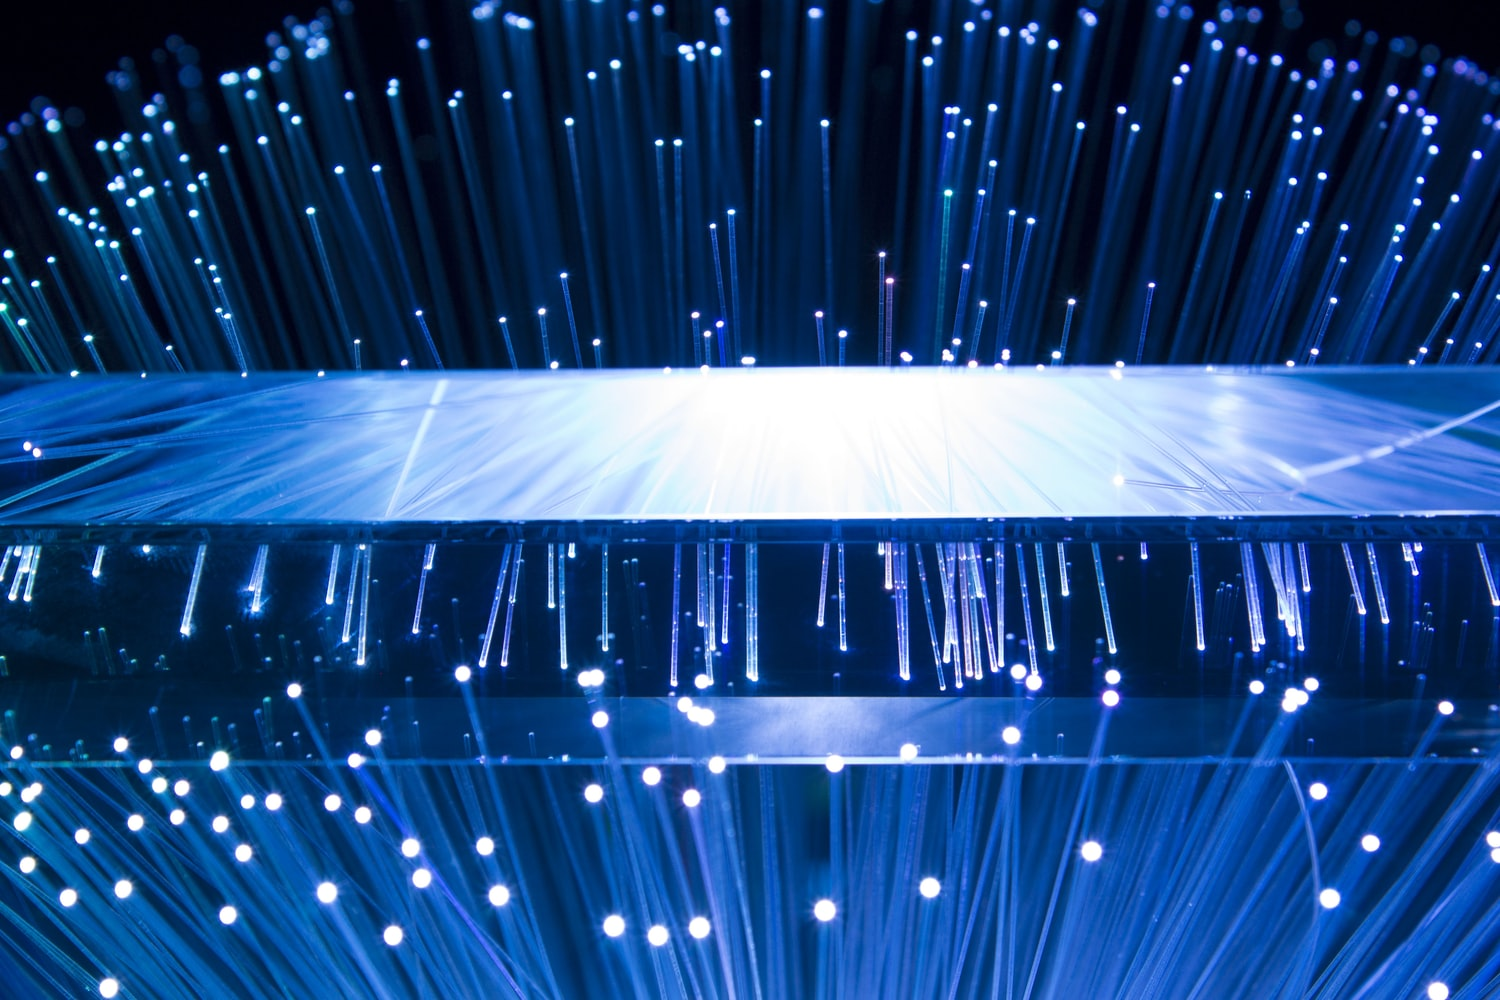
\includegraphics[width=\textwidth]{image/a}
            \caption*{Figure a}
        \end{minipage}
    \hfill
        \begin{minipage}[t]{0.3\textwidth}
            \centering
            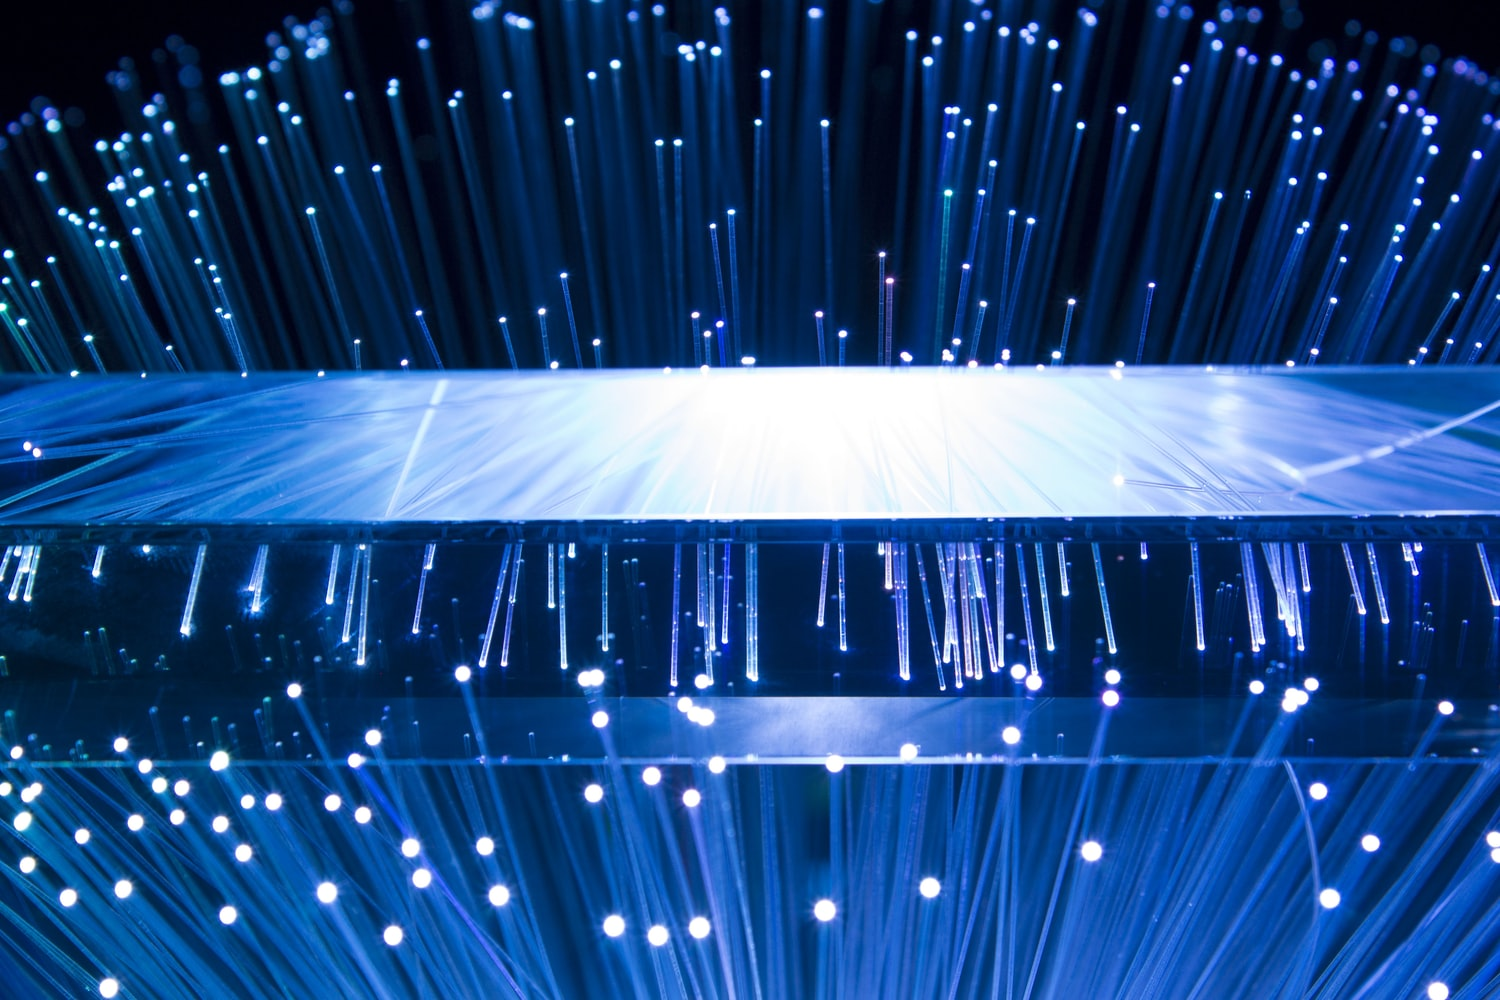
\includegraphics[width=\textwidth]{image/a}
            \caption*{Figure a}
        \end{minipage}
    \hfill
        \begin{minipage}[t]{0.3\textwidth}
            \centering
            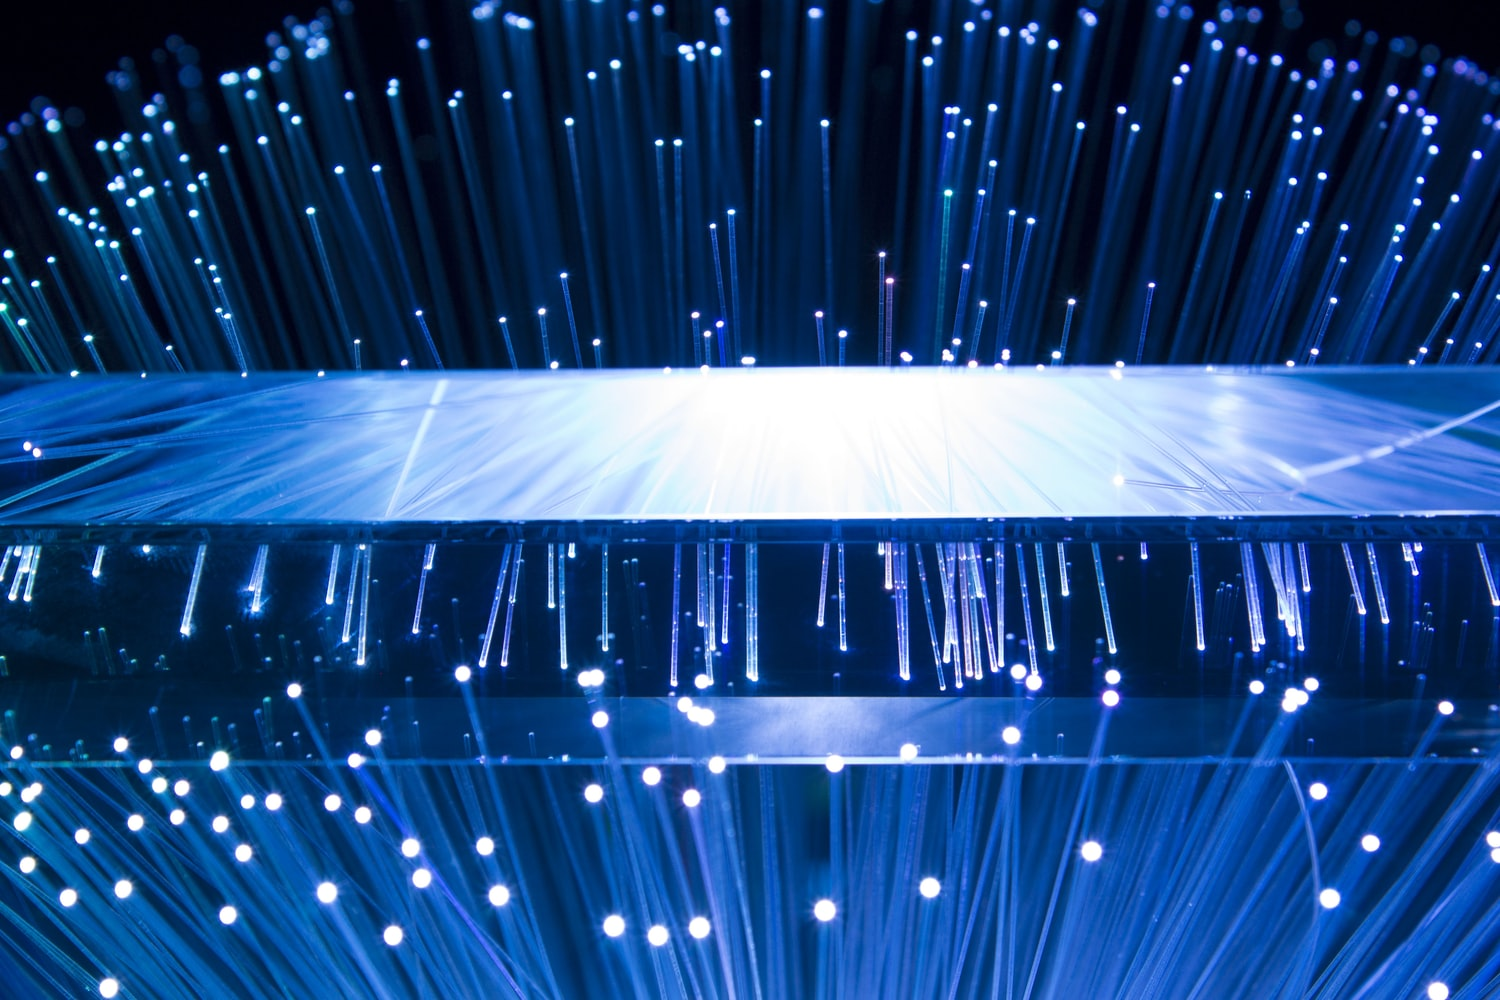
\includegraphics[width=\textwidth]{image/a}
            \caption*{Figure a}
        \end{minipage}
        
    \end{figure}
    \end{center}

\end{frame}


% New Frame
\begin{frame}{Theories 2}
\framesubtitle{Theories 2 - Section 1}
\label{P6 Theories}

Theories 2:
\begin{itemize}
\item Theories 2;
\item Theories 2;
\item Theories 2.
\end{itemize} 

\begin{center} 
        \begin{minipage}[t]{.35\textwidth}
            \centering
            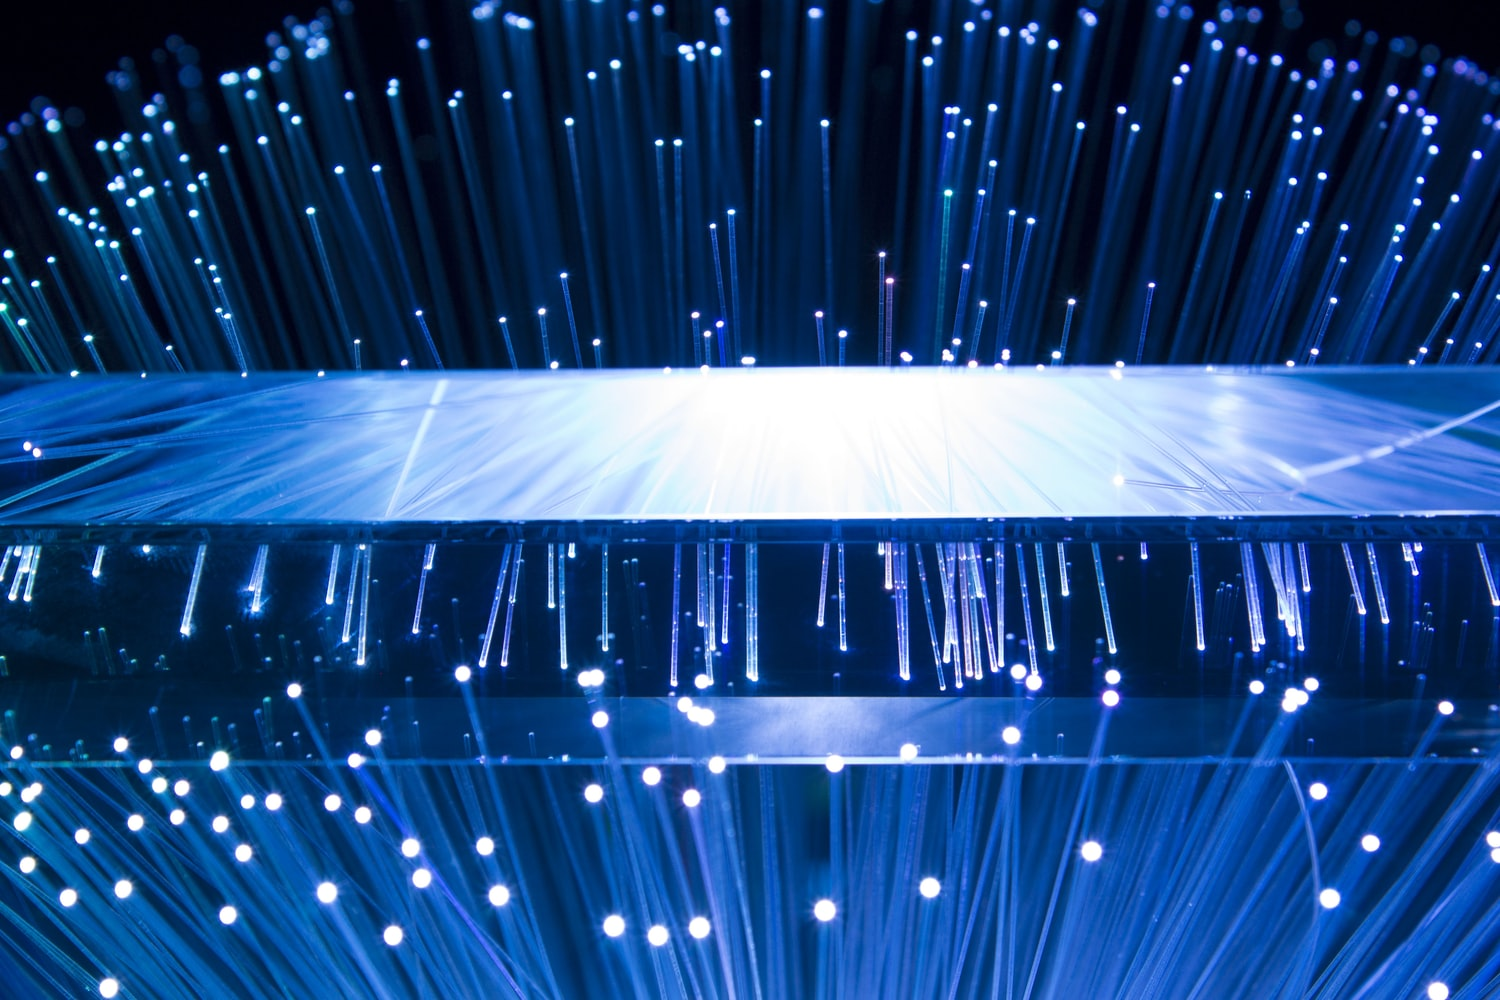
\includegraphics[height =25mm]{image/a}
            \captionof*{figure}{Figure 2}
        \end{minipage}
    \hfill
        \begin{minipage}[t]{.6\textwidth}
            \centering
            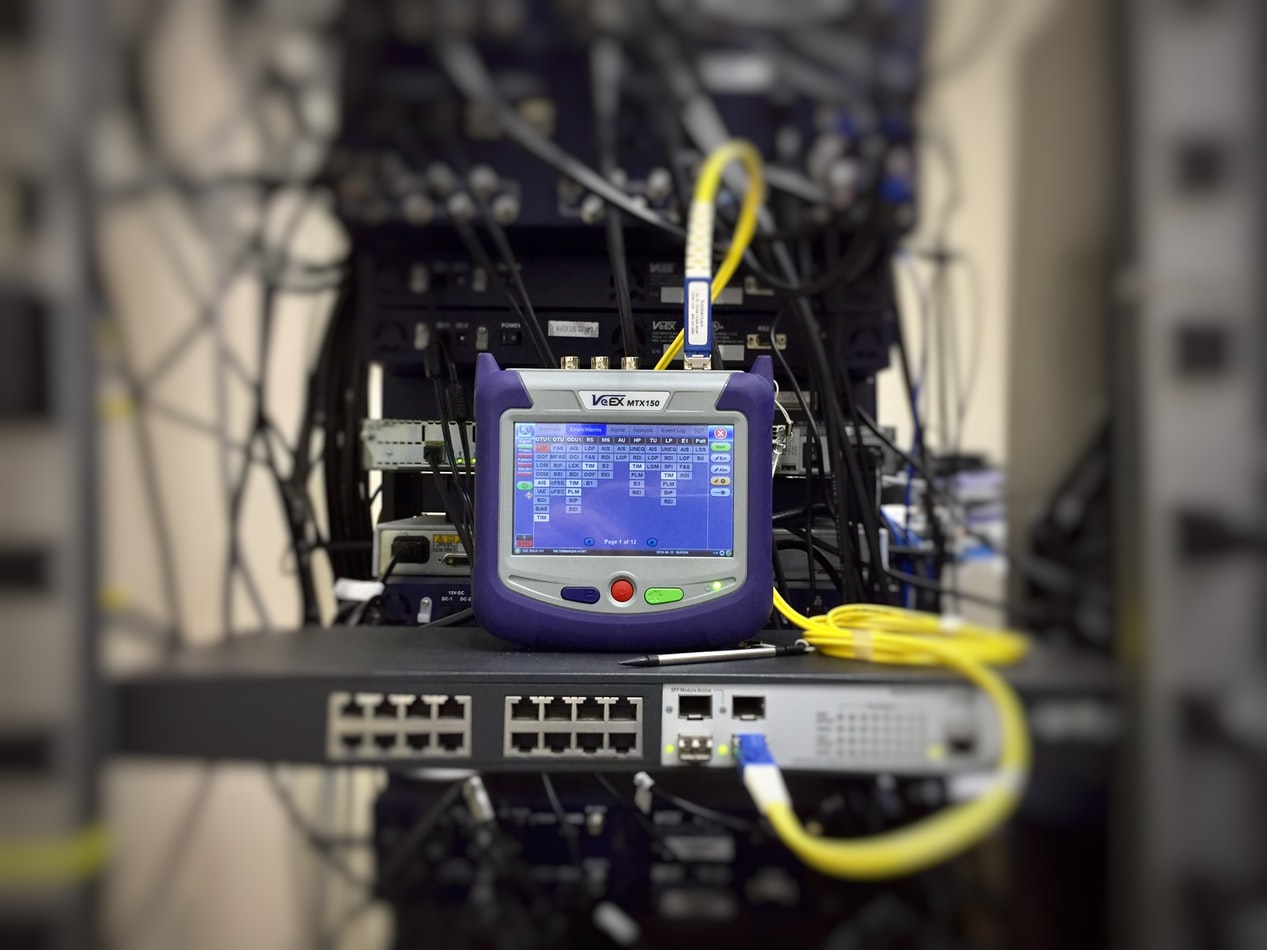
\includegraphics[height =25mm]{image/b}
            \captionof*{figure}{Figure 2}
        \end{minipage}
\end{center}

\end{frame}


% New Frame
\begin{frame}{Theories}
\framesubtitle{Theories 3}
\label{P7 Theories}

Theories Theories Theories Theories Theories Theories Theories
\vspace{30pt}

\begin{center} 
\smartdiagramset{uniform sequence color=true,
               sequence item uniform color=LUHblue!20,
               sequence item border color=black,
               sequence item border size=1pt,
               sequence item font size=\small\sffamily,}
\smartdiagram[sequence diagram]{ 
	Theories,
	A\\ "Theories", 
	Theories
}  
\end{center} 

\end{frame}


% New Frame
\begin{frame}{Conclusion}
\framesubtitle{Conclusion 1 - Section 1}
\label{P8 Conclusion}


\begin{center}


\begin{tikzpicture}[
  nonterminal/.style={
    rectangle, 
    minimum size=5mm, 
    very thick,  align=center,
    draw=red!50!black!50, 
    top color=white, % a shading that is white at the top...
    bottom color=red!50!black!20, % and something else at the bottom
    font=\itshape
  },
  terminal/.style={
    rectangle, minimum size=5mm,rounded corners=3mm,
    very thick, align=center,
    draw=black!50,
    top color=white,bottom color=black!20,
    font=\ttfamily
  },
  node distance=5mm, every on chain/.style={join}, every join/.style={->}
]

{ [start chain]
  \node [on chain,nonterminal] {Conclusion\\ Conclusion};
  \node [on chain,terminal] {A};
  \node [on chain,terminal] {B};
  \node [on chain,terminal] {C};
  \node [on chain, nonterminal] {Conclusion\\ Conclusion};
}
\end{tikzpicture}
\end{center}

\vspace{10pt}

Conclusion Conclusion Conclusion Conclusion Conclusion Conclusion

\end{frame}





% New Frame
\begin{frame}{Conclusion}
\framesubtitle{Conclusion 2}
\label{P9 Conclusion}


\begin{tiny}

\begin{table}

\centering
\caption*{Conclusion 2}
\setlength{\tabcolsep}{8mm}{

    \begin{tabular}{ccccc}% dont forget to change here
        \toprule 
            A &B &C &D &E\\
        \midrule  
            1 &1 &1 &1 &1\\
        \bottomrule 
    \end{tabular}

    \begin{tabular}{ccccc}
        \toprule 
            A &B &C &D &E\\
        \midrule  
            1 &1 &1 &1 &1\\
        \bottomrule 
    \end{tabular}}
\end{table}
\end{tiny}


\begin{tiny}
\begin{table}
\centering
\caption*{Conclusion 2}
\setlength{\tabcolsep}{8mm}{
\begin{threeparttable}
\begin{tabular}{ccccc}
     \toprule 
        A &B &C &D &E\\
    \midrule  
        1 &1 &1 &1 &1\tnote{*}\\
    \bottomrule 
\end{tabular}

\begin{tablenotes}
        \tiny
        \item[*] NOTE NOTE NOTE NOTE NOTE NOTE 
      \end{tablenotes}
    \end{threeparttable}}
\end{table}
\end{tiny}

\end{frame}


% New Frame
\begin{frame}{Outlook}
\framesubtitle{Outlook}
\label{P10 Outlook}


\begin{center}
\animategraphics[controls,width=4.2in,height=2.2in,autoplay,loop]{1}{image/d_}{001}{003}
\end{center}

\end{frame}


%References
\begin{frame}{References}
\framesubtitle{ }
\label{P35 References}

\begin{footnotesize}
	%\bibliographystyle{plain}
	\bibliographystyle{plain}
	%\bibliography{mybeamer} also works
	\bibliography{./PPT.bib}
\end{footnotesize}

\end{frame}




% End
\begin{frame}{ }
\framesubtitle{ }
\label{P36 End}

\vspace{1in}
\centering \Huge
\emph{Thank You}

\end{frame}


\end{document}